\documentclass[aspectratio=169]{ctexbeamer} 

% 极简白底黑字主题，去除多余装饰
\usetheme{default}
\usecolortheme{dove}
\setbeamertemplate{navigation symbols}{} % 隐藏右下角导航图标

\usepackage{graphicx}
\usepackage{fontspec}

\title{\Huge \textbf{No Title}}
\subtitle{\vspace{0.5em} no subtitle}
\institute{ucup-team6959 最終電車}
\author{BreakPlus}
\date{2026.7.23}

\begin{document}

% 封面
\begin{frame}
    \titlepage
\end{frame}

% 1. 与横溪大哥的对话（分两步显示）
\begin{frame}
    \vspace{2em}
    \begin{center}
        \Large
        ：“为什么我感觉 NOIp 之后世界毁灭了？”
        
        \pause % <====== 翻页后显示下一句
        
        \vspace{2.5em}
        ：“因为你脆弱。”
    \end{center}
\end{frame}

% 2. 知乎问题（图片，单页不拆分）
\begin{frame}
    \begin{center}
        
\includegraphics[width=0.85\textwidth]{1.jpg}
    \end{center}
\end{frame}

% 3. 知乎回答节选 (一) （分三步显示）
\begin{frame}
    \begin{center}
        \Large
        “因为你觉得，你本可以不这样，\\这是你能办到，却没有办到的。\\
        
        \pause % <====== 翻页后显示“你错了”
        
        \vspace{1em}
        \textbf{你错了，你本来就办不到。}”
        
        \pause % <====== 翻页后显示最后一句
        
        \vspace{2.5em}
        “不要责怪过去的自己，他真的已经尽了全力。”
    \end{center}
\end{frame}

% 4. 知乎回答节选 (二) （分两步显示）
\begin{frame}
    \begin{center}
        \large
        “不要频繁概括描绘自己的当下处境，得出一个极度悲哀的画卷图景……\\
        怨自己，是最隐蔽的怨天尤人，也是毒害最大的。”
        
        \pause % <====== 翻页后显示真正的勇士
        
        \vspace{2.5em}
        \Large
        \textbf{真正的勇士，连自己都不要怨，\\只会去想，那我现在应该做什么。}
    \end{center}
\end{frame}

% 5. WC 与 APIO 图片展示 （先显示左图，再显示右图）
\begin{frame}
    \begin{columns}
        \begin{column}{0.5\textwidth}
            \centering
            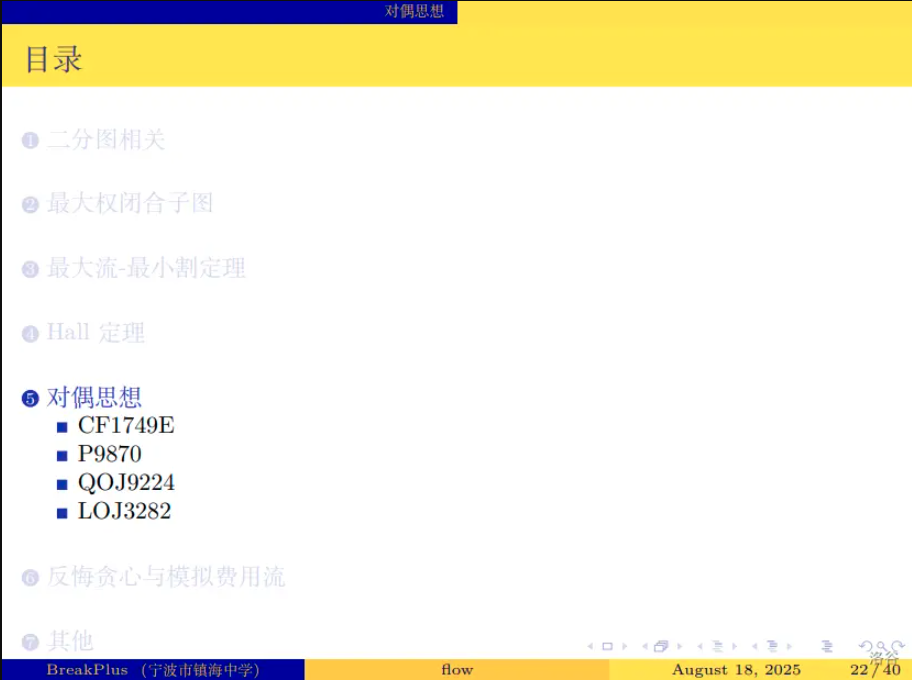
\includegraphics[width=0.95\textwidth]{2.jpg}
        \end{column}
        
        \pause % <====== 翻页后显示第二张图
        
        \begin{column}{0.5\textwidth}
            \centering
            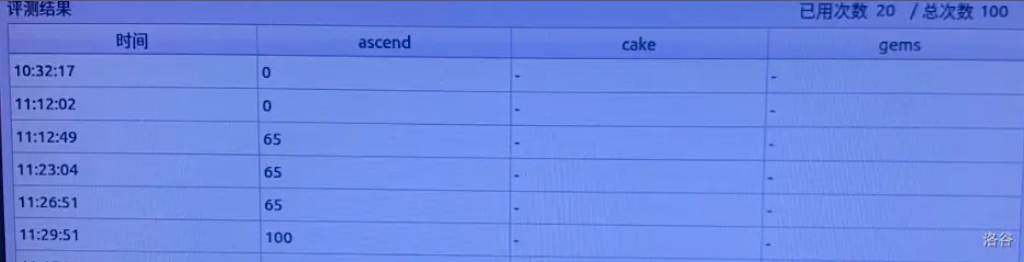
\includegraphics[width=0.95\textwidth]{3.jpg}
        \end{column}
    \end{columns}
\end{frame}

\end{document}